Escribe las coordenadas de los puntos indicados en el plano cartesiano de cada uno de los siguientes incisos.

		\begin{multicols}{2}
			\begin{parts}
				\part Coordenadas del punto A: \fillin[$(0,1)$][0in]

				\part Coordenadas del punto B: \fillin[$(3,-4)$][0in]

				\part Coordenadas del punto C: \fillin[$(2,-3)$][0in]

				\part Coordenadas del punto D: \fillin[$(0,0)$][0in]

				\part Coordenadas del punto E: \fillin[$(0,-3)$][0in]

				\part El punto B está en el cuadrante: \fillin[IV][0in]

				\part El punto C está en el cuadrante: \fillin[IV][0in]
			\end{parts}
			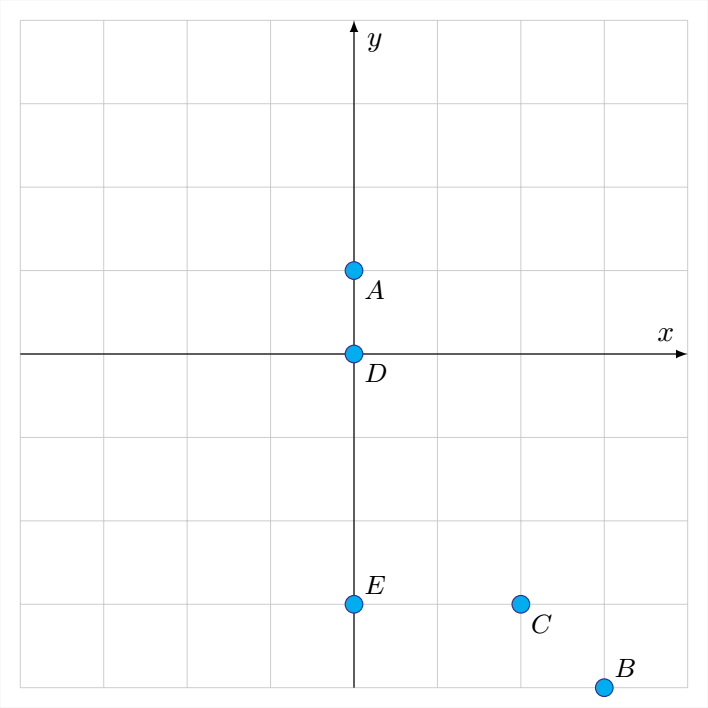
\includegraphics[width=0.75\linewidth]{../images/plano_cart01.png}
		\end{multicols}